\documentclass[12pt,a4paper]{article}

\usepackage[utf8]{inputenc}
\usepackage[T1]{fontenc}
\usepackage{amsmath,amssymb,amsfonts}
\usepackage{bm}
\usepackage{geometry}
\usepackage{graphicx}
\usepackage{hyperref}
\usepackage{tikz}
\usetikzlibrary{positioning,calc}

\geometry{margin=2.4cm}

\title{\textbf{Coherence Clusters in Multi--Subsystem Networks:\\
Emergent Domains, Interfaces, and Collective Organization}}

\author{Ivan Salines --- Independent Researcher}
\date{November 2025}

\begin{document}
\maketitle

\begin{abstract}
This chapter extends the economic field theory to networks of many interacting 
subsystems. Building on the density--phase formulation and the two-subsystem 
dynamics, we introduce the concept of a \emph{coherence cluster}: a stable 
group of subsystems whose phases evolve in unison and whose density flows 
organize into internally efficient patterns. We provide a precise operational 
definition, analyze the energy structure that drives cluster formation, 
distinguish strong-link and weak-link regimes, and show how networks naturally 
decompose into coherent economic domains. Interfaces between clusters give rise 
to tension, persistence of oscillatory modes, and long-lived metastable states. 
This framework reveals the geometry underlying economic macro-organization.
\end{abstract}

\tableofcontents

\section{Introduction}

Real economic systems are composed of many interacting subsystems: regions, 
sectors, supply chains, institutions, and strategic blocs. 
These subsystems do not evolve independently; they influence one another through 
dense, heterogeneous networks of interdependence. 

A central prediction of the economic field formulation is that such networks 
organize into \emph{coherence clusters}---groups of nodes whose phases lock 
together due to strong internal couplings. Within a cluster, tensions vanish, 
flows stabilize, and the group behaves as a single macro-entity. 
Between clusters, weaker couplings generate interfaces that support oscillations, 
misalignment, and slow relaxation.

This chapter formalizes these ideas and establishes the geometry of coherent 
organization in multi-agent economic fields.

\section{Network Structure and Interaction Geometry}

We consider a system of $N$ subsystems indexed by $i = 1,\dots,N$, connected by 
a symmetric coupling matrix 
\[
J_{ij} = J_{ji} \ge 0.
\]

Each subsystem has:
\begin{itemize}
    \item a density $\rho_i(t)$,
    \item a phase $\theta_i(t)$,
\end{itemize}
and interacts with others through the phase-dependent term in the Lagrangian:
\begin{equation}
E_{\mathrm{int}} 
= \sum_{i<j} 
  J_{ij}\,\rho_i \rho_j\,\bigl[1 - \cos(\theta_i - \theta_j)\bigr].
\label{eq:InteractionEnergy}
\end{equation}

The energetic cost of misalignment between subsystems $i$ and $j$ is proportional 
to:
\begin{equation}
J_{ij}\,\rho_i \rho_j.
\end{equation}

Thus:
\begin{itemize}
    \item pairs with \emph{large} $J_{ij}$ experience strong alignment pressure,
    \item pairs with \emph{small} $J_{ij}$ tolerate persistent misalignment.
\end{itemize}

This heterogeneity is the seed of cluster formation.

\section{Definition of a Coherence Cluster}

Let $\epsilon > 0$ be a small phase tolerance.  
A set $C \subset \{1,\dots,N\}$ is a \emph{coherence cluster} if:
\begin{enumerate}
    \item For all $i,j \in C$,
    \[
    |\theta_i(t) - \theta_j(t)| < \epsilon
    \quad \text{for } t \text{ large},
    \]
    \item For any $i \in C$ and $k \notin C$,
    \[
    J_{ik} < J_{\mathrm{int}},
    \]
    where $J_{\mathrm{int}}$ is a threshold separating strong from weak links.
\end{enumerate}

In words:
\begin{itemize}
    \item phases within the cluster lock together,
    \item the cluster is insulated from external nodes by weak links.
\end{itemize}

The threshold $J_{\mathrm{int}}$ may be defined through spectral or 
graph-theoretic properties, but at an intuitive level:
\[
J_{ij} \gg J_{ik}, J_{jk}
\quad\text{for } i,j \in C,\ k \notin C.
\]

\section{Energy Minimization and Cluster Formation}

The interaction energy~\eqref{eq:InteractionEnergy} can be decomposed into 
intra-cluster and inter-cluster contributions.

Let $C_1,\dots,C_m$ be a partition of the nodes. Then:
\begin{equation}
E_{\mathrm{int}}
= \sum_{a=1}^m \sum_{\substack{i<j\\ i,j\in C_a}}
  J_{ij}\rho_i\rho_j\,[1 - \cos(\theta_i - \theta_j)]
\quad + \quad
\sum_{\substack{i\in C_a,\, j\in C_b\\ a\neq b}}
  J_{ij}\rho_i\rho_j\,[1 - \cos(\theta_i - \theta_j)].
\end{equation}

If intra-cluster couplings satisfy:
\[
J_{ij} \gg J_{kl}
\quad\text{whenever } i,j \in C_a,\ k\in C_a,\ l \notin C_a,
\]
then minimizing $E_{\mathrm{int}}$ forces phase alignment \emph{within} each 
cluster:
\[
\theta_i \approx \theta_j 
\quad \text{for all } i,j \in C_a.
\]

Inter-cluster phases satisfy weaker constraints, allowing for:
\begin{itemize}
    \item slow drifts of relative phases,
    \item interfaces supporting oscillatory regimes,
    \item metastable non-aligned configurations.
\end{itemize}

\section{Interfaces and Weak Link Geometry}

Suppose $i\in C_a$ and $k\in C_b$ with $a\neq b$.  
If $J_{ik}$ is small, then the interaction contributes:
\[
E_{ik} \approx \tfrac{1}{2}J_{ik}\rho_i\rho_k(\Delta\theta_{ik})^2
\]
near alignment.

Thus:
\begin{itemize}
    \item misalignment costs little energy,
    \item $\theta_i$ and $\theta_k$ may oscillate relative to each other,
    \item the interface becomes a location of \emph{soft} tension.
\end{itemize}

Interfaces act as shock absorbers in the economic field.

\section{Dynamics in a Three-Cluster System}

Consider three clusters $C_1$, $C_2$, $C_3$.  
The reduced dynamics for cluster phases are approximately:
\begin{equation}
\dot{\Theta}_a
= \bar{V}_a' + \sum_{b\neq a} 
   \overline{J}_{ab}\,[1 - \cos(\Theta_a - \Theta_b)],
\end{equation}
where:
\begin{itemize}
    \item $\Theta_a$ is the common phase of cluster $C_a$,
    \item $\overline{J}_{ab}$ is the effective inter-cluster coupling,
    \item $\bar{V}_a'$ contains structural forces internal to the cluster.
\end{itemize}

This is a coarse-grained field theory on the cluster graph.

Depending on $\overline{J}_{ab}$, several regimes appear:
\begin{itemize}
    \item full global coherence ($\Theta_1=\Theta_2=\Theta_3$),
    \item partial coherence: two clusters lock, one oscillates,
    \item frustrated cycles: cyclic drift of $(\Theta_1,\Theta_2,\Theta_3)$,
    \item metastable patterns with slow reorientation.
\end{itemize}

\section{TikZ Illustration}

\begin{figure}[h]
\centering
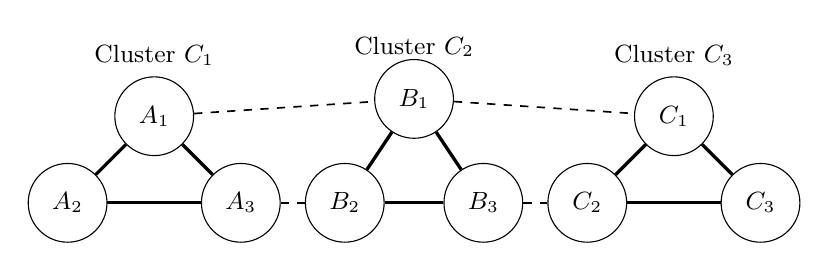
\begin{tikzpicture}[scale=1.1,
    node/.style={circle,draw,minimum size=10mm,font=\small},
    strong/.style={line width=1.2pt},
    weak/.style={line width=0.6pt,dashed}
    ]

% Cluster A (left)
\node[node] (A1) at (-3,0.8) {$A_1$};
\node[node] (A2) at (-4,-0.2) {$A_2$};
\node[node] (A3) at (-2,-0.2) {$A_3$};
\draw[strong] (A1)--(A2);
\draw[strong] (A1)--(A3);
\draw[strong] (A2)--(A3);

% Cluster B (center)
\node[node] (B1) at (0,1) {$B_1$};
\node[node] (B2) at (-0.8,-0.2) {$B_2$};
\node[node] (B3) at (0.8,-0.2) {$B_3$};
\draw[strong] (B1)--(B2);
\draw[strong] (B1)--(B3);
\draw[strong] (B2)--(B3);

% Cluster C (right)
\node[node] (C1) at (3,0.8) {$C_1$};
\node[node] (C2) at (2,-0.2) {$C_2$};
\node[node] (C3) at (4,-0.2) {$C_3$};
\draw[strong] (C1)--(C2);
\draw[strong] (C1)--(C3);
\draw[strong] (C2)--(C3);

% Weak inter-cluster links
\draw[weak] (A3)--(B2);
\draw[weak] (A1)--(B1);
\draw[weak] (B3)--(C2);
\draw[weak] (B1)--(C1);

\node at (-3,1.5) {\small Cluster $C_1$};
\node at (0,1.6) {\small Cluster $C_2$};
\node at (3,1.5) {\small Cluster $C_3$};

\end{tikzpicture}
\caption{Three coherence clusters with strong internal couplings (solid lines) 
and weak inter-cluster links (dashed lines).}
\end{figure}

\section{Summary}

Multi-subsystem networks naturally organize into coherence clusters due to the 
heterogeneous structure of interdependence. 
Within each cluster, strong couplings enforce phase alignment and stable density 
flows. 
Between clusters, weak links create interfaces that support oscillatory modes, 
metastability, and slow relaxation.

Cluster formation is an emergent geometric phenomenon: it arises from the 
minimization of interaction energy and the dynamics of the density--phase field, 
not from external constraints or imposed structure.

This chapter prepares the ground for the analysis of oscillatory regimes, global 
coherence, and economic phase transitions in the next chapters.

\end{document}
